

\documentclass{article}


\title{Grid pattern formation}
\author{Simone Poetto}
\date{March 2020}

\usepackage{textcomp}
\usepackage{graphicx}
\usepackage{float}
\usepackage{subfig}


\begin{document}


\maketitle

\section{Code Description}
Description of the code from \cite{Sorscher}
\subsection{Place cells}

Place cell centers are randomly and uniformly distribuited throughout the environment (square box 2.2x2.2).

\begin{figure}[H]
\centering
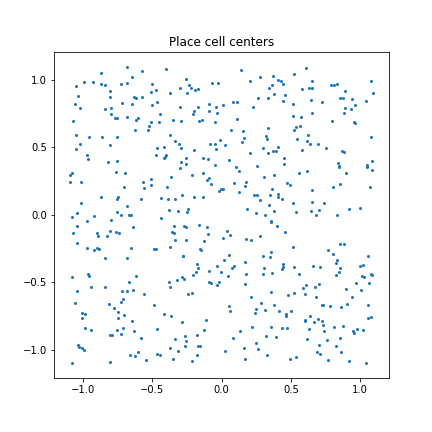
\includegraphics[scale=0.6]{images/place_cell_centers.png}
\label{placecells}
\end{figure}

\bigskip

\subsection{Trajectories}
Trajectory are generated according to \cite{traj}

The rat uses first order motion dynamics, i.e. constant speed and no acceleration. It can detect and avoid obstacles by a limited line-of-sight mechanism.

Here are some sample trajectory generated inside the square arena:
\begin{figure}[H]
\centering
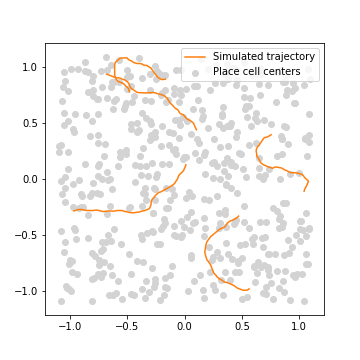
\includegraphics[scale=0.5]{images/trajectories.png}
\label{trajectory}
\end{figure}

\subsection{Place cells activation}
Here is an exemple of the place cells activations for a single trajectory at different time step.

\begin{figure}[H]
\centering
\subfloat[][Trajectory]
	{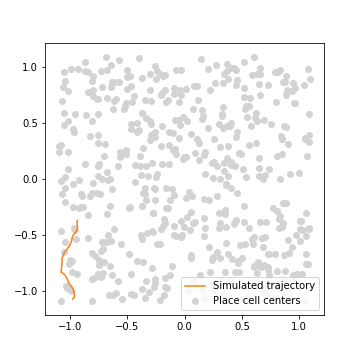
\includegraphics[scale=0.38]{images/trajectory.png}}
\subfloat[][Activations]
	{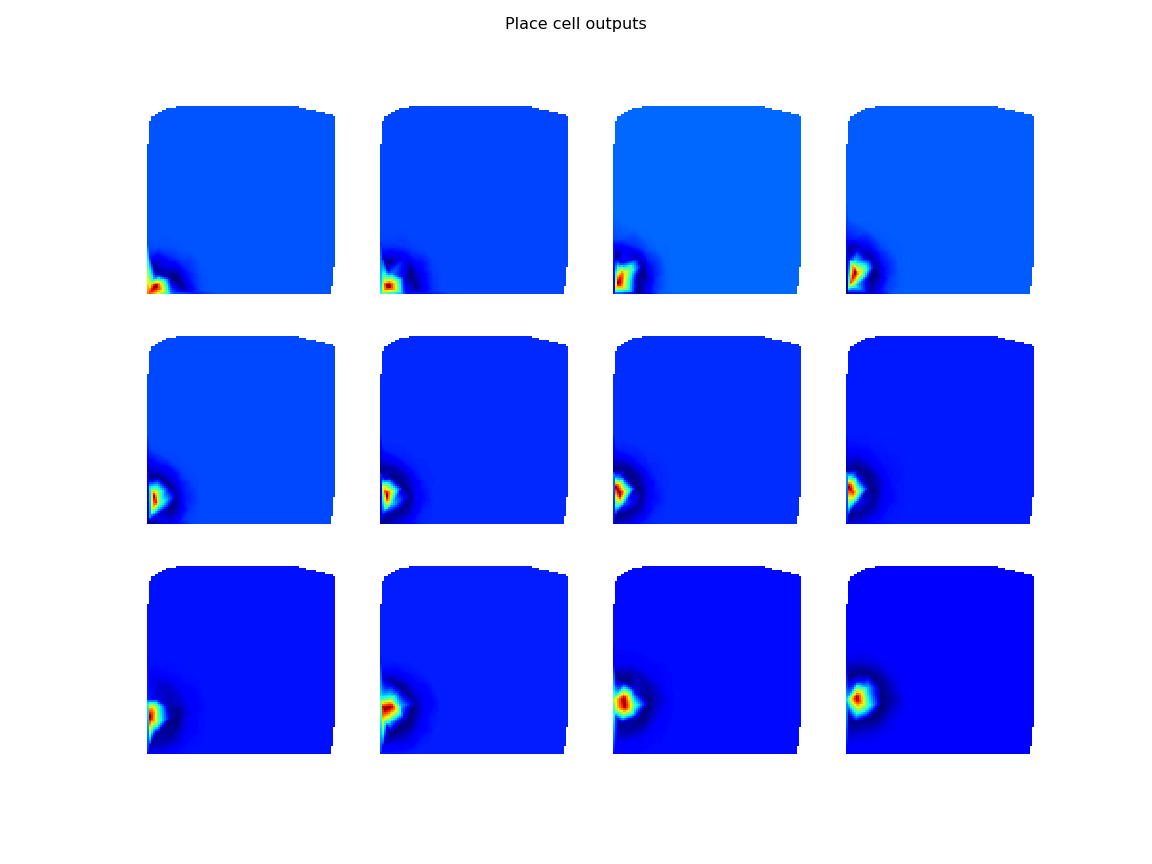
\includegraphics[scale=0.18]{images/pcoutput.png}}
\end{figure}


The response of the i-th place cell is simulated either using a gaussian or a difference of gaussians.

\subsection{Place cells covariance}

Here is the place cells covariance for both cases: response modulated by a gaussian or by a difference of gaussians:

 \begin{figure}[H]
\centering
\subfloat[][Gaussian]
	{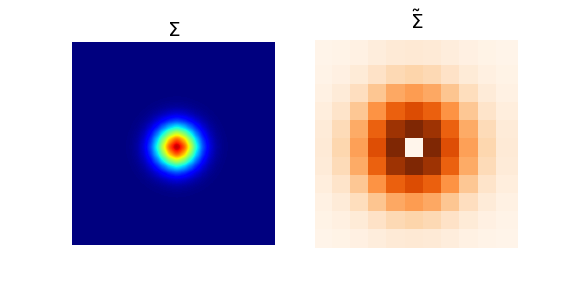
\includegraphics[scale=0.35]{images/gauss.png}}
\subfloat[][Diffence of gaussians]
	{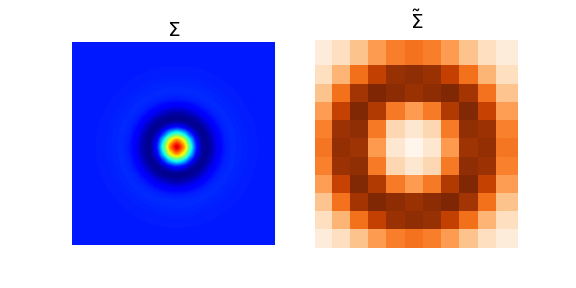
\includegraphics[scale=0.35]{images/dog.png}}
\end{figure}



\bigskip
\bibliographystyle{plain}
\bibliography{bibliography}

\end{document}

}

